\documentclass{article}

\usepackage[letterpaper, margin=1in]{geometry}

\usepackage{titlesec}
%\usepackage[none]{hyphenat} % use only if there is a problem
% Use Unicode characters
\usepackage[utf8]{inputenc}

% tables
\usepackage{longtable,booktabs,array}
\usepackage{multirow}
\usepackage{afterpage}

% figures
\usepackage{wrapfig}
\usepackage{lscape}
\usepackage{rotating}
\usepackage{graphicx}
\graphicspath{assets}
\usepackage{times}
\usepackage{caption}
\usepackage{float}
\floatstyle{plaintop}
\restylefloat{table}

\title{Supplementary material for "Gut-resident microorganisms and their genes are associated with cognition and neuroanatomy in children"}

\begin{document}

\baselineskip24pt

\maketitle

\begin{figure}[h]
    \centering
    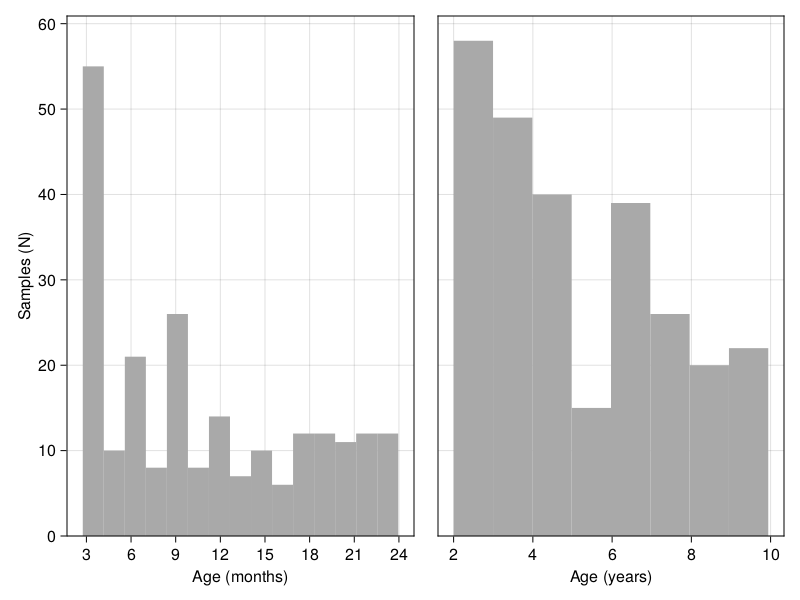
\includegraphics[width=0.9\textwidth]{assets/Supp_Figure1.png}
    \captionsetup{labelformat=empty}
    \caption{
        \textbf{Figure S1: The age of participants when samples were collected is weighted towards early times.} Sample collection by age - related to Figure 1A. A histogram showing the number of samples
        included in this study by the age of the child when the sample was collected.
    }
\end{figure}

\begin{figure}[h]
    \centering
    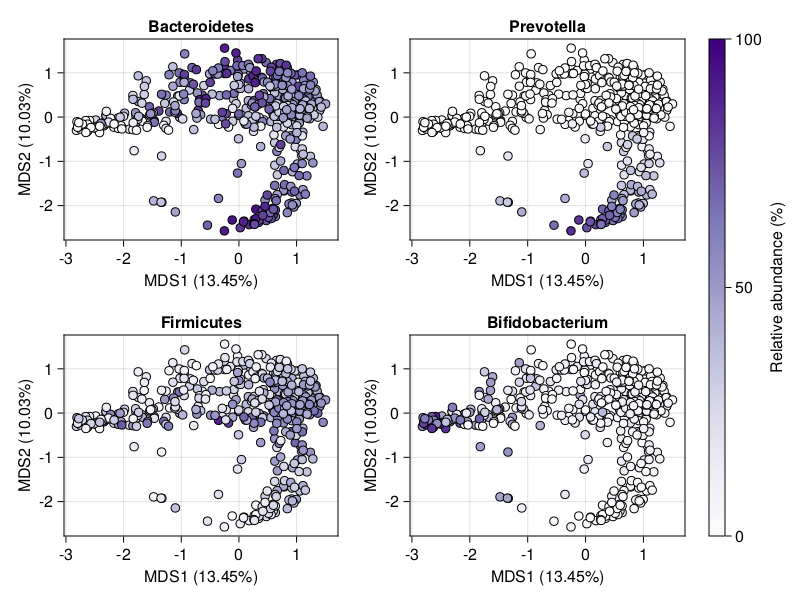
\includegraphics[width=0.9\textwidth]{assets/Supp_Figure2.png}
    \captionsetup{labelformat=empty}
    \caption{
        \textbf{Figure S2: The broad pattern microbial beta diversity is consonant with previous studies.} Principal coordinates analysis of taxonomic profiles - 
        related to Figure 1C. PCoAs are colored by the relative abundance per-sample
        of major phyla (Bacteroidetes, top left; Firmicutes, bottom left)
        and genera (\textit{Prevotella}, top right; \textit{Bifidobacterium}, bottom right).
    }
\end{figure}

\begin{figure}[h]
    \centering
    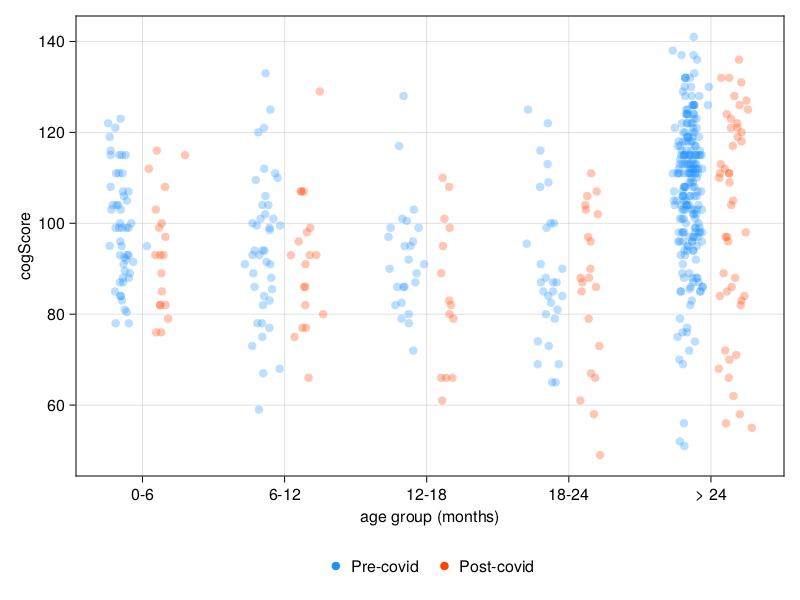
\includegraphics[width=0.9\textwidth]{assets/Supp_Figure3.png}
    \captionsetup{labelformat=empty}
    \caption{
        \textbf{Figure S3: Cognitive assessment scores declined during COVID-19}. Scores in red were collected after March of 2020.
    }
\end{figure}

\begin{figure}[h]
  \centering
  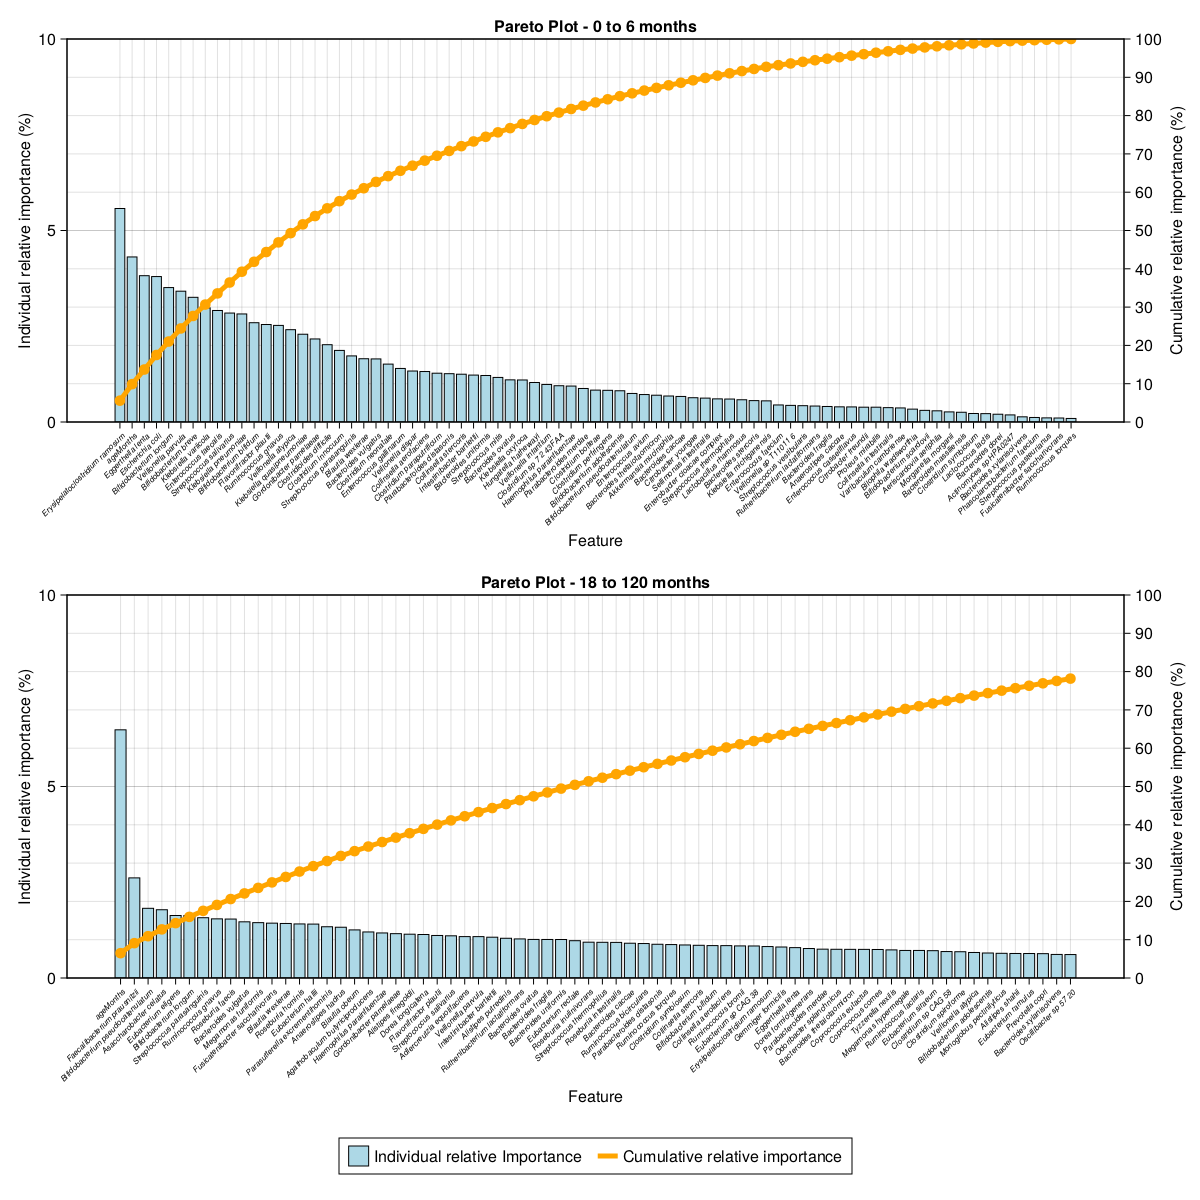
\includegraphics[width=0.9\textwidth]{assets/Supp_Figure4.png}
  \captionsetup{labelformat=empty}
  \caption{
      \textbf{Figure S4}: Pareto plots for RFs of cognitive function - related to Figure 3C-D.
      The cumulative importance (orange line), as well as ranked importance (blue bars)
      of features (species) in models of cogntive performance score
      in children from birth to 6 months (top) or
      in children from 18 to 120 months (bottom).
  }
\end{figure}

\begin{figure}[h]
  \centering
  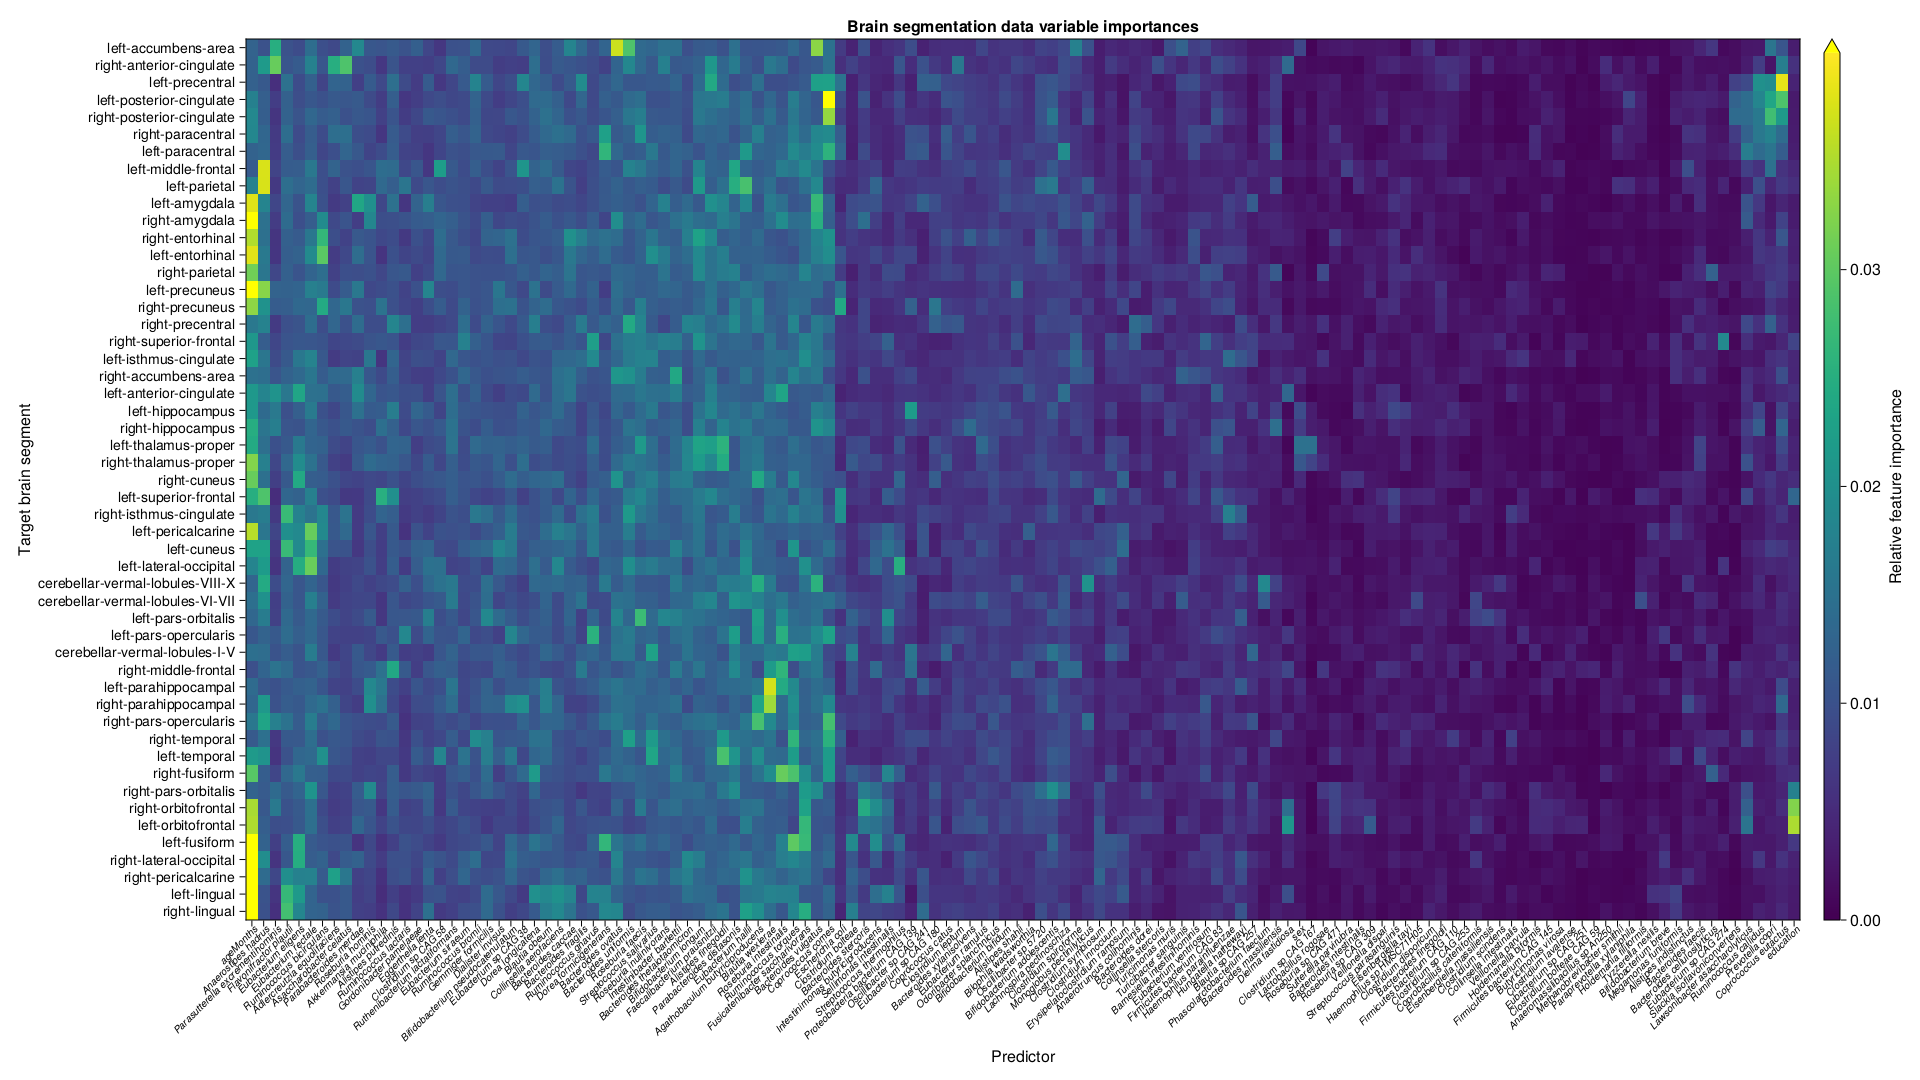
\includegraphics[width=0.9\textwidth]{assets/Supp_Figure5.png}
  \captionsetup{labelformat=empty}
  \caption{
      \textbf{Figure S5}: Heatmap of feature importances for each brain region -
      related to Figure 4B. This heatmap contains all features included in models
      (including age) and all brain segments. Importance values over 0.04
      are colored white.
  }
\end{figure}

\begin{sidewaysfigure}[h]
  \centering
  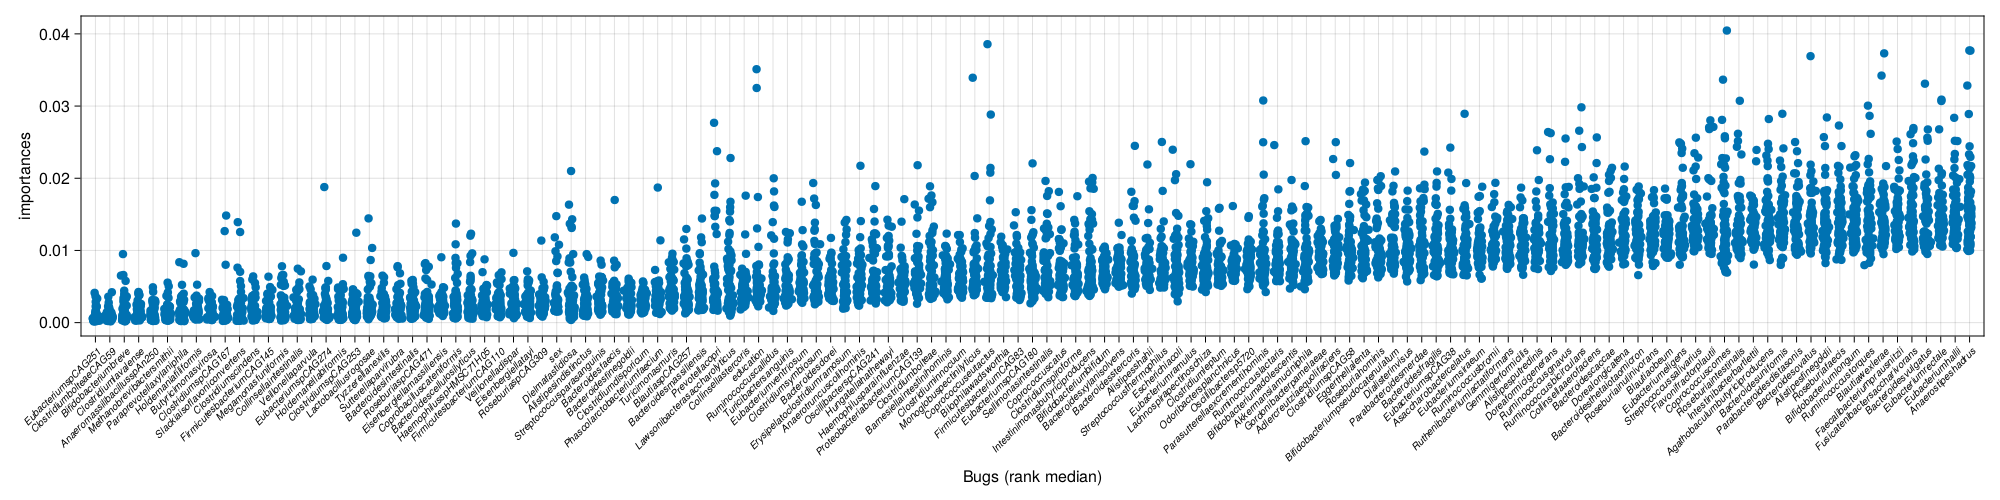
\includegraphics[width=0.9\textwidth]{assets/Supp_Figure6.png}
  \captionsetup{labelformat=empty}
  \caption{
      \textbf{Figure S6}: Species feature importances in brain region RFs - related to Figure 4C.
      All species (plus sex and maternal education) feature importances in each brain region model.
      X-axis is rank-ordered by median importance across all brain region models.
  }
\end{sidewaysfigure}

\begin{figure}[h]
  \centering
  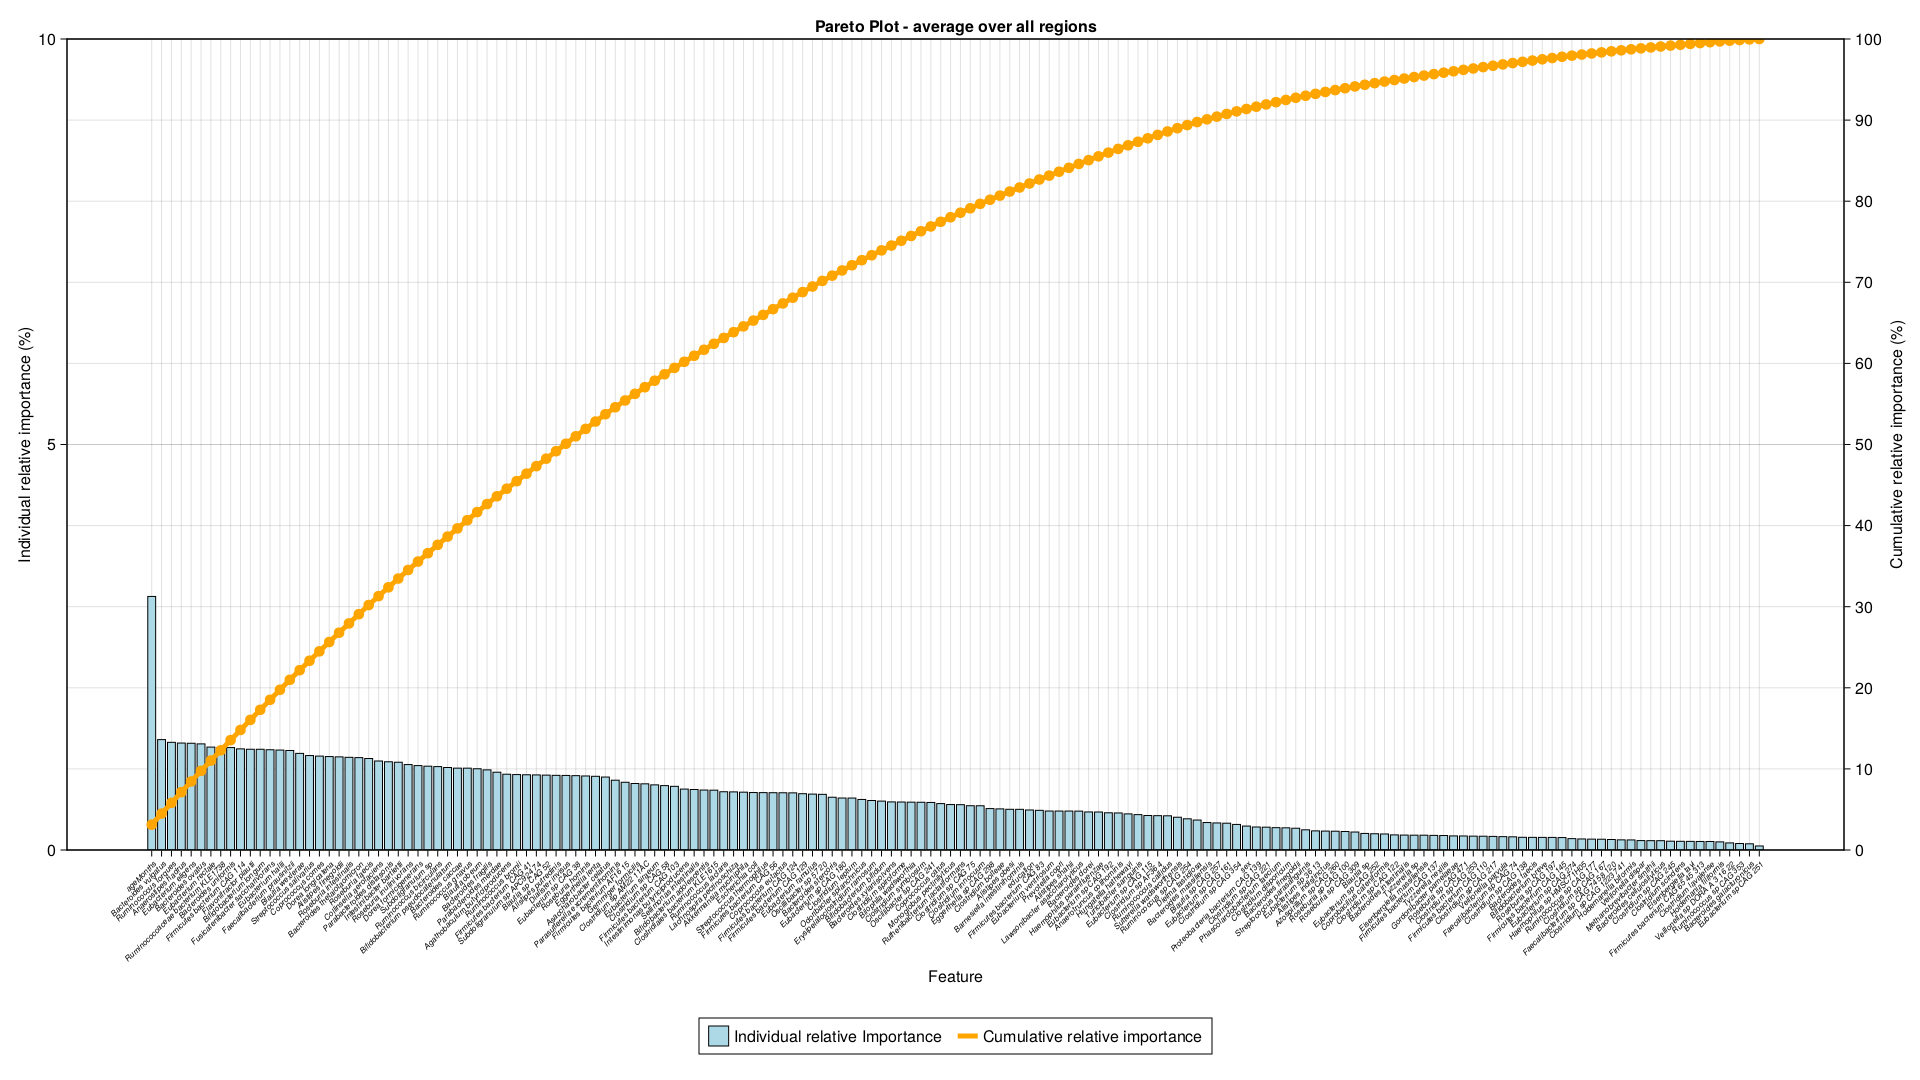
\includegraphics[width=0.9\textwidth]{assets/Supp_Figure7.png}
  \captionsetup{labelformat=empty}
  \caption{
      \textbf{Figure S7}: Pareto plots for RFs of cognitive function - related to Figure 4.
      The cumulative average importance (orange line), as well as ranked average importance (blue bars)
      of features (species) in models of brain region size.
  }
\end{figure}


\begin{table}[h]
     \begin{centering}
      \tiny
  \begin{tabular}{|r|r|r|r|r|}
      \hline
      \textbf{rank} & \textbf{variable} & \textbf{weightedImportance} & \textbf{relativeWeightedImportance} & \textbf{cumulativeWeightedImportance} \\\hline
      1 & \textit{ageMonths} & 0.01907 & 5.99 \% & 5.99 \% \\
      2 & \textit{Faecalibacterium prausnitzii} & 0.00701 & 2.2 \% & 8.19 \% \\
      3 & \textit{Blautia wexlerae} & 0.00534 & 1.68 \% & 9.87 \% \\
      4 & \textit{Eubacterium eligens} & 0.00505 & 1.59 \% & 11.45 \% \\
      5 & \textit{Bifidobacterium pseudocatenulatum} & 0.00501 & 1.57 \% & 13.03 \% \\
      6 & \textit{Bifidobacterium longum} & 0.00484 & 1.52 \% & 14.55 \% \\
      7 & \textit{Veillonella dispar} & 0.00454 & 1.43 \% & 15.97 \% \\
      8 & \textit{Parasutterella excrementihominis} & 0.00438 & 1.38 \% & 17.35 \% \\
      9 & \textit{Bacteroides vulgatus} & 0.004 & 1.26 \% & 18.61 \% \\
      10 & \textit{Roseburia faecis} & 0.00397 & 1.25 \% & 19.85 \% \\
      11 & \textit{Fusicatenibacter saccharivorans} & 0.00385 & 1.21 \% & 21.06 \% \\
      12 & \textit{Eubacterium hallii} & 0.00361 & 1.13 \% & 22.2 \% \\
      13 & \textit{Anaerostipes hadrus} & 0.00358 & 1.12 \% & 23.32 \% \\
      14 & \textit{Asaccharobacter celatus} & 0.00355 & 1.12 \% & 24.43 \% \\
      15 & \textit{Dorea longicatena} & 0.00351 & 1.1 \% & 25.54 \% \\
      16 & \textit{Blautia obeum} & 0.00347 & 1.09 \% & 26.63 \% \\
      17 & \textit{Ruminococcus gnavus} & 0.00345 & 1.08 \% & 27.71 \% \\
      18 & \textit{Flavonifractor plautii} & 0.00338 & 1.06 \% & 28.77 \% \\
      19 & \textit{Intestinibacter bartlettii} & 0.00336 & 1.06 \% & 29.83 \% \\
      20 & \textit{Veillonella parvula} & 0.00335 & 1.05 \% & 30.88 \% \\
      21 & \textit{Roseburia hominis} & 0.00335 & 1.05 \% & 31.93 \% \\
      22 & \textit{Alistipes obesi} & 0.00326 & 1.02 \% & 32.95 \% \\
      23 & \textit{Eubacterium sp CAG 38} & 0.00323 & 1.01 \% & 33.97 \% \\
      24 & \textit{Parabacteroides distasonis} & 0.00321 & 1.01 \% & 34.98 \% \\
      25 & \textit{Streptococcus parasanguinis} & 0.00321 & 1.01 \% & 35.98 \% \\
      26 & \textit{Megamonas funiformis} & 0.00314 & 0.99 \% & 36.97 \% \\
      27 & \textit{Bifidobacterium bifidum} & 0.00309 & 0.97 \% & 37.94 \% \\
      28 & \textit{Streptococcus salivarius} & 0.00303 & 0.95 \% & 38.89 \% \\
      29 & \textit{Roseburia intestinalis} & 0.00303 & 0.95 \% & 39.84 \% \\
      30 & \textit{Sutterella wadsworthensis} & 0.00301 & 0.95 \% & 40.79 \% \\
      31 & \textit{Eubacterium rectale} & 0.00297 & 0.93 \% & 41.72 \% \\
      32 & \textit{Alistipes finegoldii} & 0.00294 & 0.92 \% & 42.64 \% \\
      33 & \textit{Bacteroides uniformis} & 0.0029 & 0.91 \% & 43.55 \% \\
      34 & \textit{Parabacteroides merdae} & 0.00288 & 0.91 \% & 44.46 \% \\
      35 & \textit{Roseburia inulinivorans} & 0.00287 & 0.9 \% & 45.36 \% \\
      36 & \textit{Firmicutes bacterium CAG 41} & 0.00287 & 0.9 \% & 46.26 \% \\
      37 & \textit{Veillonella atypica} & 0.00285 & 0.89 \% & 47.16 \% \\
      38 & \textit{Bacteroides ovatus} & 0.00277 & 0.87 \% & 48.03 \% \\
      39 & \textit{Haemophilus parainfluenzae} & 0.00277 & 0.87 \% & 48.9 \% \\
      40 & \textit{Subdoligranulum sp} & 0.00276 & 0.87 \% & 49.77 \% \\
      41 & \textit{Bacteroides caccae} & 0.00272 & 0.86 \% & 50.62 \% \\
      42 & \textit{Alistipes putredinis} & 0.00267 & 0.84 \% & 51.46 \% \\
      43 & \textit{Monoglobus pectinilyticus} & 0.00259 & 0.81 \% & 52.27 \% \\
      44 & \textit{Anaerotruncus colihominis} & 0.00259 & 0.81 \% & 53.09 \% \\
      45 & \textit{Clostridium sp CAG 58} & 0.00258 & 0.81 \% & 53.9 \% \\
      46 & \textit{Subdoligranulum sp APC924 74} & 0.00258 & 0.81 \% & 54.71 \% \\
      47 & \textit{Collinsella aerofaciens} & 0.00256 & 0.8 \% & 55.51 \% \\
      48 & \textit{Eggerthella lenta} & 0.00255 & 0.8 \% & 56.31 \% \\
      49 & \textit{Bacteroides fragilis} & 0.00252 & 0.79 \% & 57.1 \% \\
      50 & \textit{Ruthenibacterium lactatiformans} & 0.0025 & 0.78 \% & 57.89 \% \\
      51 & \textit{Streptococcus thermophilus} & 0.00246 & 0.77 \% & 58.66 \% \\
      52 & \textit{Ruminococcus torques} & 0.00246 & 0.77 \% & 59.44 \% \\
      53 & \textit{Ruminococcus bromii} & 0.00235 & 0.74 \% & 60.17 \% \\
      54 & \textit{Clostridium symbiosum} & 0.00232 & 0.73 \% & 60.9 \% \\
      55 & \textit{Agathobaculum butyriciproducens} & 0.00231 & 0.73 \% & 61.63 \% \\
      56 & \textit{Firmicutes bacterium AF16 15} & 0.00227 & 0.71 \% & 62.34 \% \\
      57 & \textit{Ruminococcus bicirculans} & 0.00225 & 0.71 \% & 63.05 \% \\
      58 & \textit{Prevotella copri} & 0.00224 & 0.7 \% & 63.75 \% \\
      59 & \textit{Bacteroides thetaiotaomicron} & 0.00223 & 0.7 \% & 64.45 \% \\
      60 & \textit{Bifidobacterium adolescentis} & 0.00223 & 0.7 \% & 65.15 \% \\
      61 & \textit{Ruminococcus lactaris} & 0.00219 & 0.69 \% & 65.84 \% \\
      62 & \textit{Eubacterium ramulus} & 0.00215 & 0.68 \% & 66.51 \% \\
      63 & \textit{Odoribacter splanchnicus} & 0.00214 & 0.67 \% & 67.19 \% \\
      64 & \textit{Dorea formicigenerans} & 0.00213 & 0.67 \% & 67.85 \% \\
      65 & \textit{Eubacterium siraeum} & 0.00211 & 0.66 \% & 68.52 \% \\
      66 & \textit{Erysipelatoclostridium ramosum} & 0.00208 & 0.65 \% & 69.17 \% \\
      67 & \textit{Ruminococcaceae bacterium KLE1738} & 0.00207 & 0.65 \% & 69.82 \% \\
      68 & \textit{Sellimonas intestinalis} & 0.00205 & 0.64 \% & 70.46 \% \\
      69 & \textit{Clostridium sp AM22 11AC} & 0.00201 & 0.63 \% & 71.1 \% \\
      70 & \textit{Firmicutes bacterium CAG 114} & 0.00193 & 0.61 \% & 71.7 \% \\
      71 & \textit{Clostridium leptum} & 0.00191 & 0.6 \% & 72.31 \% \\
      72 & \textit{Oscillibacter sp 57 20} & 0.00187 & 0.59 \% & 72.89 \% \\
      73 & \textit{Eubacterium sp CAG 180} & 0.00187 & 0.59 \% & 73.48 \% \\
      74 & \textit{Gemmiger formicilis} & 0.00182 & 0.57 \% & 74.05 \% \\
      75 & \textit{Bacteroides xylanisolvens} & 0.00181 & 0.57 \% & 74.62 \% \\
      76 & \textit{Blautia sp CAG 52} & 0.00176 & 0.55 \% & 75.17 \% \\
      77 & \textit{Bacteroides dorei} & 0.00175 & 0.55 \% & 75.72 \% \\
      78 & \textit{Hungatella hathewayi} & 0.00173 & 0.54 \% & 76.27 \% \\
      79 & \textit{Intestinimonas butyriciproducens} & 0.00172 & 0.54 \% & 76.81 \% \\
      80 & \textit{Akkermansia muciniphila} & 0.00172 & 0.54 \% & 77.35 \% \\
      81 & \textit{Clostridium innocuum} & 0.0017 & 0.54 \% & 77.88 \% \\
      82 & \textit{Clostridium spiroforme} & 0.00169 & 0.53 \% & 78.41 \% \\
      83 & \textit{Clostridium bolteae} & 0.00168 & 0.53 \% & 78.94 \% \\
      84 & \textit{Coprococcus comes} & 0.00164 & 0.52 \% & 79.46 \% \\
      85 & \textit{Bifidobacterium breve} & 0.00161 & 0.51 \% & 79.96 \% \\
      86 & \textit{Escherichia coli} & 0.00159 & 0.5 \% & 80.46 \% \\
      87 & \textit{Eggerthella sp CAG 298} & 0.00155 & 0.49 \% & 80.95 \% \\
      88 & \textit{Dialister invisus} & 0.00155 & 0.49 \% & 81.44 \% \\
      89 & \textit{Clostridium sp CAG 75} & 0.00154 & 0.48 \% & 81.92 \% \\
      90 & \textit{Coprococcus eutactus} & 0.00154 & 0.48 \% & 82.4 \% \\
      91 & \textit{Bacteroides stercoris} & 0.00152 & 0.48 \% & 82.88 \% \\
      92 & \textit{Tyzzerella nexilis} & 0.00152 & 0.48 \% & 83.36 \% \\
      93 & \textit{Lachnospira pectinoschiza} & 0.00151 & 0.47 \% & 83.83 \% \\
      94 & \textit{Clostridium citroniae} & 0.00144 & 0.45 \% & 84.28 \% \\
      95 & \textit{Eubacterium sp 36 13} & 0.00142 & 0.45 \% & 84.73 \% \\
      96 & \textit{Bilophila wadsworthia} & 0.00142 & 0.45 \% & 85.18 \% \\
      97 & \textit{Firmicutes bacterium CAG 56} & 0.0014 & 0.44 \% & 85.62 \% \\
      98 & \textit{Ruminococcus sp CAG 353} & 0.00139 & 0.44 \% & 86.05 \% \\
      99 & \textit{Firmicutes bacterium CAG 129} & 0.00138 & 0.43 \% & 86.49 \% \\
      100 & \textit{Eisenbergiella massiliensis} & 0.00131 & 0.41 \% & 86.9 \% \\
      101 & \textit{Barnesiella intestinihominis} & 0.0013 & 0.41 \% & 87.3 \% \\
      102 & \textit{Clostridium sp AF36 4} & 0.0013 & 0.41 \% & 87.71 \% \\
      103 & \textit{Clostridiales bacterium KLE1615} & 0.00123 & 0.39 \% & 88.1 \% \\
      104 & \textellipsis & \textellipsis & \textellipsis  & \textellipsis \\\hline
    \end{tabular}
    \caption*{
      \textbf{Table S1}: Feature importances for RF models of cognitive performance
      based on taxonomic profiles in children over 18 months old.
  }
  \end{centering}
\end{table}


\begin{table}
  \begin{centering}
    \tiny
\begin{tabular}{|r|r|r|r|r|}
  \hline
  \textbf{rank} & \textbf{variable} & \textbf{weightedImportance} & \textbf{relativeWeightedImportance} & \textbf{cumulativeWeightedImportance} \\\hline
  1 & \textit{Bifidobacterium pseudocatenulatum} & 0.0082 & 3.55 \% & 3.55 \% \\
  2 & \textit{ageMonths} & 0.00765 & 3.31 \% & 6.87 \% \\
  3 & \textit{Blautia wexlerae} & 0.0061 & 2.64 \% & 9.51 \% \\
  4 & \textit{Eubacterium eligens} & 0.00502 & 2.18 \% & 11.68 \% \\
  5 & \textit{Faecalibacterium prausnitzii} & 0.00499 & 2.16 \% & 13.85 \% \\
  6 & \textit{Bifidobacterium longum} & 0.00402 & 1.74 \% & 15.59 \% \\
  7 & \textit{Ruminococcus gnavus} & 0.00352 & 1.52 \% & 17.11 \% \\
  8 & \textit{Fusicatenibacter saccharivorans} & 0.00324 & 1.41 \% & 18.52 \% \\
  9 & \textit{Roseburia inulinivorans} & 0.0031 & 1.34 \% & 19.86 \% \\
  10 & \textit{Flavonifractor plautii} & 0.00309 & 1.34 \% & 21.2 \% \\
  11 & \textit{Intestinibacter bartlettii} & 0.00302 & 1.31 \% & 22.51 \% \\
  12 & \textit{Anaerostipes hadrus} & 0.00293 & 1.27 \% & 23.78 \% \\
  13 & \textit{Streptococcus salivarius} & 0.00291 & 1.26 \% & 25.03 \% \\
  14 & \textit{Parasutterella excrementihominis} & 0.00286 & 1.24 \% & 26.27 \% \\
  15 & \textit{Veillonella parvula} & 0.00283 & 1.23 \% & 27.5 \% \\
  16 & \textit{Bilophila wadsworthia} & 0.0027 & 1.17 \% & 28.67 \% \\
  17 & \textit{Eggerthella lenta} & 0.00269 & 1.17 \% & 29.84 \% \\
  18 & \textit{Veillonella dispar} & 0.00258 & 1.12 \% & 30.95 \% \\
  19 & \textit{Roseburia intestinalis} & 0.00256 & 1.11 \% & 32.06 \% \\
  20 & \textit{Eubacterium rectale} & 0.00255 & 1.1 \% & 33.16 \% \\
  21 & \textit{Bacteroides uniformis} & 0.00253 & 1.09 \% & 34.26 \% \\
  22 & \textit{Bacteroides fragilis} & 0.00252 & 1.09 \% & 35.35 \% \\
  23 & \textit{Streptococcus thermophilus} & 0.00251 & 1.09 \% & 36.44 \% \\
  24 & \textit{Bacteroides vulgatus} & 0.00249 & 1.08 \% & 37.52 \% \\
  25 & \textit{Roseburia faecis} & 0.00248 & 1.08 \% & 38.59 \% \\
  26 & \textit{Blautia sp CAG 52} & 0.00244 & 1.06 \% & 39.65 \% \\
  27 & \textit{Parabacteroides distasonis} & 0.00239 & 1.03 \% & 40.68 \% \\
  28 & \textit{Ruminococcus bromii} & 0.00232 & 1.0 \% & 41.69 \% \\
  29 & \textit{Roseburia hominis} & 0.00231 & 1.0 \% & 42.69 \% \\
  30 & \textit{Clostridium sp CAG 58} & 0.0023 & 1.0 \% & 43.69 \% \\
  31 & \textit{Intestinimonas butyriciproducens} & 0.00224 & 0.97 \% & 44.66 \% \\
  32 & \textit{Bacteroides ovatus} & 0.00216 & 0.93 \% & 45.59 \% \\
  33 & \textit{Veillonella atypica} & 0.00213 & 0.92 \% & 46.51 \% \\
  34 & \textit{Erysipelatoclostridium ramosum} & 0.00212 & 0.92 \% & 47.43 \% \\
  35 & \textit{Alistipes shahii} & 0.00212 & 0.92 \% & 48.35 \% \\
  36 & \textit{Barnesiella intestinihominis} & 0.00209 & 0.91 \% & 49.26 \% \\
  37 & \textit{Clostridium symbiosum} & 0.00208 & 0.9 \% & 50.16 \% \\
  38 & \textit{Ruthenibacterium lactatiformans} & 0.00207 & 0.9 \% & 51.05 \% \\
  39 & \textit{Collinsella aerofaciens} & 0.00201 & 0.87 \% & 51.92 \% \\
  40 & \textit{Firmicutes bacterium CAG 41} & 0.002 & 0.87 \% & 52.79 \% \\
  41 & \textit{Bacteroides xylanisolvens} & 0.00194 & 0.84 \% & 53.63 \% \\
  42 & \textit{Hungatella hathewayi} & 0.00194 & 0.84 \% & 54.47 \% \\
  43 & \textit{Firmicutes bacterium AF16 15} & 0.00191 & 0.83 \% & 55.29 \% \\
  44 & \textit{Anaerotruncus colihominis} & 0.0019 & 0.82 \% & 56.12 \% \\
  45 & \textit{Clostridium bolteae} & 0.00189 & 0.82 \% & 56.94 \% \\
  46 & \textit{Haemophilus parainfluenzae} & 0.00185 & 0.8 \% & 57.74 \% \\
  47 & \textit{Bacteroides caccae} & 0.00184 & 0.8 \% & 58.54 \% \\
  48 & \textit{Alistipes putredinis} & 0.00181 & 0.79 \% & 59.32 \% \\
  49 & \textit{Agathobaculum butyriciproducens} & 0.00181 & 0.78 \% & 60.11 \% \\
  50 & \textit{Streptococcus parasanguinis} & 0.00179 & 0.78 \% & 60.88 \% \\
  51 & \textit{Blautia obeum} & 0.00176 & 0.76 \% & 61.64 \% \\
  52 & \textit{Eubacterium hallii} & 0.00175 & 0.76 \% & 62.4 \% \\
  53 & \textit{Parabacteroides merdae} & 0.00175 & 0.76 \% & 63.16 \% \\
  54 & \textit{Sutterella wadsworthensis} & 0.00174 & 0.76 \% & 63.92 \% \\
  55 & \textit{Eubacterium sp CAG 38} & 0.00173 & 0.75 \% & 64.67 \% \\
  56 & \textit{Alistipes finegoldii} & 0.0017 & 0.74 \% & 65.4 \% \\
  57 & \textit{Escherichia coli} & 0.00169 & 0.73 \% & 66.14 \% \\
  58 & \textit{Sellimonas intestinalis} & 0.00168 & 0.73 \% & 66.86 \% \\
  59 & \textit{Bacteroides thetaiotaomicron} & 0.00167 & 0.72 \% & 67.59 \% \\
  60 & \textit{Ruminococcus torques} & 0.00166 & 0.72 \% & 68.3 \% \\
  61 & \textit{Ruminococcus lactaris} & 0.00162 & 0.7 \% & 69.01 \% \\
  62 & \textit{Ruminococcaceae bacterium KLE1738} & 0.00159 & 0.69 \% & 69.7 \% \\
  63 & \textit{Firmicutes bacterium CAG 114} & 0.00158 & 0.68 \% & 70.38 \% \\
  64 & \textit{Clostridium innocuum} & 0.00156 & 0.68 \% & 71.06 \% \\
  65 & \textit{Clostridium clostridioforme} & 0.00156 & 0.68 \% & 71.73 \% \\
  66 & \textit{Megamonas funiformis} & 0.00155 & 0.67 \% & 72.4 \% \\
  67 & \textit{Asaccharobacter celatus} & 0.00152 & 0.66 \% & 73.06 \% \\
  68 & \textit{Subdoligranulum sp} & 0.00151 & 0.66 \% & 73.72 \% \\
  69 & \textit{Dialister invisus} & 0.0015 & 0.65 \% & 74.37 \% \\
  70 & \textit{Clostridium sp AM22 11AC} & 0.00148 & 0.64 \% & 75.01 \% \\
  71 & \textit{Dorea longicatena} & 0.00147 & 0.64 \% & 75.65 \% \\
  72 & \textit{Bifidobacterium bifidum} & 0.00147 & 0.64 \% & 76.29 \% \\
  73 & \textit{Lachnospira pectinoschiza} & 0.0014 & 0.61 \% & 76.89 \% \\
  74 & \textit{Ruminococcus sp CAG 254} & 0.00139 & 0.6 \% & 77.5 \% \\
  75 & \textit{Dorea formicigenerans} & 0.00138 & 0.6 \% & 78.09 \% \\
  76 & \textit{Blautia sp CAG 257} & 0.00137 & 0.6 \% & 78.69 \% \\
  77 & \textit{Bifidobacterium breve} & 0.00133 & 0.58 \% & 79.27 \% \\
  78 & \textit{Eubacterium siraeum} & 0.00133 & 0.58 \% & 79.84 \% \\
  79 & \textit{Akkermansia muciniphila} & 0.0013 & 0.56 \% & 80.41 \% \\
  80 & \textit{Bifidobacterium adolescentis} & 0.0013 & 0.56 \% & 80.97 \% \\
  81 & \textit{Anaerostipes caccae} & 0.00124 & 0.54 \% & 81.51 \% \\
  82 & \textit{Clostridium sp CAG 122} & 0.00124 & 0.54 \% & 82.04 \% \\
  83 & \textit{Clostridium sp CAG 75} & 0.00122 & 0.53 \% & 82.57 \% \\
  84 & \textit{Eubacterium sp CAG 180} & 0.00122 & 0.53 \% & 83.1 \% \\
  85 & \textit{Firmicutes bacterium CAG 56} & 0.00121 & 0.52 \% & 83.62 \% \\
  86 & \textit{Ruminococcus bicirculans} & 0.00119 & 0.52 \% & 84.14 \% \\
  87 & \textit{Odoribacter splanchnicus} & 0.00112 & 0.49 \% & 84.62 \% \\
  88 & \textit{Clostridium lavalense} & 0.00108 & 0.47 \% & 85.09 \% \\
  89 & \textit{Clostridium sp CAG 12237 41} & 0.00107 & 0.46 \% & 85.56 \% \\
  90 & \textit{Alistipes obesi} & 0.00107 & 0.46 \% & 86.02 \% \\
  91 & \textit{Clostridium spiroforme} & 0.00103 & 0.45 \% & 86.46 \% \\
  92 & \textit{Bacteroides stercoris} & 0.00096 & 0.42 \% & 86.88 \% \\
  93 & \textit{Tyzzerella nexilis} & 0.00094 & 0.41 \% & 87.29 \% \\
  94 & \textit{Clostridium leptum} & 0.00094 & 0.41 \% & 87.69 \% \\
  95 & \textit{Eggerthella sp CAG 298} & 0.00091 & 0.39 \% & 88.09 \% \\
  96 & \textit{Eisenbergiella massiliensis} & 0.00088 & 0.38 \% & 88.47 \% \\
  97 & \textit{Subdoligranulum sp APC924 74} & 0.00085 & 0.37 \% & 88.84 \% \\
  98 & \textit{Clostridium citroniae} & 0.00085 & 0.37 \% & 89.21 \% \\
  99 & \textit{Bacteroides dorei} & 0.00084 & 0.37 \% & 89.57 \% \\
  100 & \textit{Eubacterium sp CAG 252} & 0.00082 & 0.36 \% & 89.93 \% \\
  101 & \textit{Turicibacter sanguinis} & 0.00079 & 0.34 \% & 90.27 \% \\
  102 & \textit{Gemmiger formicilis} & 0.00078 & 0.34 \% & 90.61 \% \\
  103 & \textit{Phascolarctobacterium faecium} & 0.00076 & 0.33 \% & 90.94 \% \\
  104 & \textellipsis & \textellipsis & \textellipsis  & \textellipsis \\\hline
\end{tabular}
\caption*{
  \textbf{Table S2}: Feature importances for RF models of MSEL expressive language
  based on taxonomic profiles in children over 18 months old.
}
\end{centering}
\end{table}

\begin{table}
  \begin{centering}
    \tiny
\begin{tabular}{|r|r|r|r|r|}
  \hline
  \textbf{rank} & \textbf{variable} & \textbf{weightedImportance} & \textbf{relativeWeightedImportance} & \textbf{cumulativeWeightedImportance} \\\hline
  1 & \textit{ageMonths} & 0.00679 & 4.58 \% & 4.58 \% \\
  2 & \textit{Roseburia faecis} & 0.00358 & 2.41 \% & 6.99 \% \\
  3 & \textit{Blautia wexlerae} & 0.00277 & 1.87 \% & 8.85 \% \\
  4 & \textit{Streptococcus salivarius} & 0.00274 & 1.85 \% & 10.7 \% \\
  5 & \textit{Faecalibacterium prausnitzii} & 0.00264 & 1.78 \% & 12.48 \% \\
  6 & \textit{Fusicatenibacter saccharivorans} & 0.00249 & 1.68 \% & 14.15 \% \\
  7 & \textit{Clostridium symbiosum} & 0.00238 & 1.6 \% & 15.76 \% \\
  8 & \textit{Bifidobacterium longum} & 0.00231 & 1.55 \% & 17.31 \% \\
  9 & \textit{Subdoligranulum sp} & 0.00221 & 1.49 \% & 18.8 \% \\
  10 & \textit{Ruminococcus gnavus} & 0.00219 & 1.47 \% & 20.27 \% \\
  11 & \textit{Bifidobacterium pseudocatenulatum} & 0.00218 & 1.47 \% & 21.74 \% \\
  12 & \textit{Ruminococcus bromii} & 0.00218 & 1.47 \% & 23.21 \% \\
  13 & \textit{Firmicutes bacterium CAG 41} & 0.00216 & 1.45 \% & 24.66 \% \\
  14 & \textit{Bacteroides uniformis} & 0.00216 & 1.45 \% & 26.12 \% \\
  15 & \textit{Eubacterium sp CAG 252} & 0.00207 & 1.39 \% & 27.51 \% \\
  16 & \textit{Intestinibacter bartlettii} & 0.00199 & 1.34 \% & 28.85 \% \\
  17 & \textit{Anaerostipes hadrus} & 0.00195 & 1.31 \% & 30.16 \% \\
  18 & \textit{Flavonifractor plautii} & 0.00194 & 1.31 \% & 31.47 \% \\
  19 & \textit{Clostridiales bacterium KLE1615} & 0.00189 & 1.28 \% & 32.75 \% \\
  20 & \textit{Parabacteroides distasonis} & 0.00189 & 1.27 \% & 34.02 \% \\
  21 & \textit{Ruminococcus torques} & 0.00178 & 1.2 \% & 35.22 \% \\
  22 & \textit{Collinsella aerofaciens} & 0.00177 & 1.19 \% & 36.41 \% \\
  23 & \textit{Eubacterium sp CAG 38} & 0.00173 & 1.17 \% & 37.58 \% \\
  24 & \textit{Roseburia intestinalis} & 0.0017 & 1.15 \% & 38.73 \% \\
  25 & \textit{Erysipelatoclostridium ramosum} & 0.00167 & 1.13 \% & 39.86 \% \\
  26 & \textit{Coprococcus catus} & 0.00167 & 1.12 \% & 40.98 \% \\
  27 & \textit{Bacteroides fragilis} & 0.00164 & 1.11 \% & 42.09 \% \\
  28 & \textit{Clostridium innocuum} & 0.00161 & 1.09 \% & 43.17 \% \\
  29 & \textit{Clostridium sp CAG 75} & 0.00161 & 1.08 \% & 44.26 \% \\
  30 & \textit{Eubacterium eligens} & 0.00157 & 1.06 \% & 45.31 \% \\
  31 & \textit{Ruminococcus bicirculans} & 0.00156 & 1.05 \% & 46.37 \% \\
  32 & \textit{Dorea formicigenerans} & 0.00156 & 1.05 \% & 47.42 \% \\
  33 & \textit{Escherichia coli} & 0.00153 & 1.03 \% & 48.45 \% \\
  34 & \textit{Bacteroides thetaiotaomicron} & 0.00152 & 1.03 \% & 49.48 \% \\
  35 & \textit{Eggerthella lenta} & 0.00152 & 1.02 \% & 50.5 \% \\
  36 & \textit{Sellimonas intestinalis} & 0.00151 & 1.01 \% & 51.51 \% \\
  37 & \textit{Alistipes putredinis} & 0.00147 & 0.99 \% & 52.51 \% \\
  38 & \textit{Bacteroides ovatus} & 0.00147 & 0.99 \% & 53.5 \% \\
  39 & \textit{Eubacterium rectale} & 0.00146 & 0.99 \% & 54.49 \% \\
  40 & \textit{Bacteroides vulgatus} & 0.00145 & 0.98 \% & 55.47 \% \\
  41 & \textit{Roseburia inulinivorans} & 0.0014 & 0.94 \% & 56.41 \% \\
  42 & \textit{Parasutterella excrementihominis} & 0.0014 & 0.94 \% & 57.35 \% \\
  43 & \textit{Agathobaculum butyriciproducens} & 0.00137 & 0.92 \% & 58.28 \% \\
  44 & \textit{Clostridium bolteae} & 0.00135 & 0.91 \% & 59.19 \% \\
  45 & \textit{Ruminococcus lactaris} & 0.00132 & 0.89 \% & 60.08 \% \\
  46 & \textit{Firmicutes bacterium CAG 56} & 0.0013 & 0.88 \% & 60.96 \% \\
  47 & \textit{Ruthenibacterium lactatiformans} & 0.0013 & 0.88 \% & 61.83 \% \\
  48 & \textit{Eubacterium hallii} & 0.00129 & 0.87 \% & 62.7 \% \\
  49 & \textit{Coprococcus comes} & 0.00122 & 0.82 \% & 63.53 \% \\
  50 & \textit{Bifidobacterium bifidum} & 0.00121 & 0.81 \% & 64.34 \% \\
  51 & \textit{Bilophila wadsworthia} & 0.00119 & 0.8 \% & 65.15 \% \\
  52 & \textit{Hungatella hathewayi} & 0.00116 & 0.78 \% & 65.93 \% \\
  53 & \textit{Haemophilus parainfluenzae} & 0.00114 & 0.77 \% & 66.7 \% \\
  54 & \textit{Streptococcus thermophilus} & 0.00114 & 0.77 \% & 67.47 \% \\
  55 & \textit{Bacteroides caccae} & 0.00111 & 0.75 \% & 68.21 \% \\
  56 & \textit{Clostridium sp AM22 11AC} & 0.0011 & 0.74 \% & 68.96 \% \\
  57 & \textit{Roseburia hominis} & 0.0011 & 0.74 \% & 69.69 \% \\
  58 & \textit{Blautia obeum} & 0.00108 & 0.73 \% & 70.42 \% \\
  59 & \textit{Ruminococcus sp CAG 254} & 0.00105 & 0.71 \% & 71.13 \% \\
  60 & \textit{Firmicutes bacterium AF16 15} & 0.00103 & 0.7 \% & 71.83 \% \\
  61 & \textit{Alistipes finegoldii} & 0.001 & 0.67 \% & 72.5 \% \\
  62 & \textit{Megamonas funiformis} & 0.00089 & 0.6 \% & 73.1 \% \\
  63 & \textit{Intestinimonas butyriciproducens} & 0.00089 & 0.6 \% & 73.7 \% \\
  64 & \textit{Blautia sp CAG 257} & 0.00086 & 0.58 \% & 74.27 \% \\
  65 & \textit{Anaerotruncus colihominis} & 0.00084 & 0.57 \% & 74.84 \% \\
  66 & \textit{Gemmiger formicilis} & 0.00084 & 0.57 \% & 75.41 \% \\
  67 & \textit{Dielma fastidiosa} & 0.00083 & 0.56 \% & 75.97 \% \\
  68 & \textit{Subdoligranulum sp APC924 74} & 0.00083 & 0.56 \% & 76.53 \% \\
  69 & \textit{Dorea longicatena} & 0.00082 & 0.55 \% & 77.08 \% \\
  70 & \textit{Bifidobacterium adolescentis} & 0.00082 & 0.55 \% & 77.63 \% \\
  71 & \textit{Clostridium sp CAG 58} & 0.00081 & 0.55 \% & 78.18 \% \\
  72 & \textit{Clostridium lavalense} & 0.00079 & 0.53 \% & 78.71 \% \\
  73 & \textit{Clostridium leptum} & 0.00078 & 0.53 \% & 79.24 \% \\
  74 & \textit{Bacteroides stercoris} & 0.00078 & 0.53 \% & 79.77 \% \\
  75 & \textit{Clostridium sp CAG 122} & 0.00078 & 0.53 \% & 80.29 \% \\
  76 & \textit{Eubacterium ramulus} & 0.00078 & 0.52 \% & 80.82 \% \\
  77 & \textit{Holdemania filiformis} & 0.00077 & 0.52 \% & 81.34 \% \\
  78 & \textit{Eubacterium sp 36 13} & 0.00077 & 0.52 \% & 81.86 \% \\
  79 & \textit{Ruminococcaceae bacterium KLE1738} & 0.00077 & 0.52 \% & 82.38 \% \\
  80 & \textit{Firmicutes bacterium CAG 114} & 0.00076 & 0.52 \% & 82.89 \% \\
  81 & \textit{Clostridium sp CAG 12237 41} & 0.00076 & 0.51 \% & 83.41 \% \\
  82 & \textit{Lachnospira pectinoschiza} & 0.00075 & 0.51 \% & 83.91 \% \\
  83 & \textit{Parabacteroides merdae} & 0.00072 & 0.49 \% & 84.4 \% \\
  84 & \textit{Dialister invisus} & 0.00071 & 0.48 \% & 84.88 \% \\
  85 & \textit{Eisenbergiella massiliensis} & 0.00068 & 0.46 \% & 85.34 \% \\
  86 & \textit{Streptococcus parasanguinis} & 0.00067 & 0.45 \% & 85.79 \% \\
  87 & \textit{Turicibacter sanguinis} & 0.00067 & 0.45 \% & 86.24 \% \\
  88 & \textit{Akkermansia muciniphila} & 0.00066 & 0.44 \% & 86.68 \% \\
  89 & \textit{Tyzzerella nexilis} & 0.00064 & 0.43 \% & 87.11 \% \\
  90 & \textit{Clostridium aldenense} & 0.00062 & 0.42 \% & 87.53 \% \\
  91 & \textit{Bacteroides dorei} & 0.00062 & 0.41 \% & 87.95 \% \\
  92 & \textit{Clostridium spiroforme} & 0.0006 & 0.4 \% & 88.35 \% \\
  93 & \textit{Phascolarctobacterium faecium} & 0.00058 & 0.39 \% & 88.74 \% \\
  94 & \textit{Bacteroides xylanisolvens} & 0.00058 & 0.39 \% & 89.13 \% \\
  95 & \textit{Bifidobacterium breve} & 0.00057 & 0.39 \% & 89.52 \% \\
  96 & \textit{Veillonella dispar} & 0.00055 & 0.37 \% & 89.89 \% \\
  97 & \textit{Eubacterium siraeum} & 0.00054 & 0.36 \% & 90.25 \% \\
  98 & \textit{Asaccharobacter celatus} & 0.00053 & 0.36 \% & 90.61 \% \\
  99 & \textit{Clostridium sp CAG 354} & 0.00053 & 0.36 \% & 90.97 \% \\
  100 & \textit{Prevotella copri} & 0.00048 & 0.32 \% & 91.29 \% \\
  101 & \textit{Coprococcus eutactus} & 0.00047 & 0.32 \% & 91.61 \% \\
  102 & \textit{Odoribacter splanchnicus} & 0.00045 & 0.31 \% & 91.92 \% \\
  103 & \textit{Oscillibacter sp 57 20} & 0.00044 & 0.3 \% & 92.21 \% \\
  104 & \textellipsis & \textellipsis & \textellipsis  & \textellipsis \\\hline
\end{tabular}
\caption*{
  \textbf{Table S3}: Feature importances for RF models of MSEL gross motor
  based on taxonomic profiles in children over 18 months old.
  }
\end{centering}
\end{table}

\begin{table}
  \begin{centering}
    \tiny
\begin{tabular}{|r|r|r|r|r|}
  \hline
  \textbf{rank} & \textbf{variable} & \textbf{weightedImportance} & \textbf{relativeWeightedImportance} & \textbf{cumulativeWeightedImportance} \\\hline
  1 & \textit{ageMonths} & 0.01081 & 4.69 \% & 4.69 \% \\
  2 & \textit{Faecalibacterium prausnitzii} & 0.00534 & 2.32 \% & 7.01 \% \\
  3 & \textit{Bifidobacterium pseudocatenulatum} & 0.00394 & 1.71 \% & 8.72 \% \\
  4 & \textit{Roseburia faecis} & 0.00391 & 1.7 \% & 10.42 \% \\
  5 & \textit{Clostridium innocuum} & 0.00385 & 1.67 \% & 12.09 \% \\
  6 & \textit{Bacteroides vulgatus} & 0.00379 & 1.64 \% & 13.73 \% \\
  7 & \textit{Blautia wexlerae} & 0.00374 & 1.62 \% & 15.35 \% \\
  8 & \textit{Bifidobacterium longum} & 0.00371 & 1.61 \% & 16.96 \% \\
  9 & \textit{Parabacteroides merdae} & 0.00334 & 1.45 \% & 18.41 \% \\
  10 & \textit{Eubacterium sp CAG 38} & 0.00329 & 1.43 \% & 19.84 \% \\
  11 & \textit{Intestinibacter bartlettii} & 0.00314 & 1.36 \% & 21.2 \% \\
  12 & \textit{Anaerostipes hadrus} & 0.00299 & 1.3 \% & 22.5 \% \\
  13 & \textit{Megamonas funiformis} & 0.00286 & 1.24 \% & 23.74 \% \\
  14 & \textit{Eggerthella lenta} & 0.0027 & 1.17 \% & 24.91 \% \\
  15 & \textit{Eubacterium eligens} & 0.00265 & 1.15 \% & 26.06 \% \\
  16 & \textit{Ruminococcus bromii} & 0.00261 & 1.13 \% & 27.2 \% \\
  17 & \textit{Ruminococcus gnavus} & 0.00261 & 1.13 \% & 28.33 \% \\
  18 & \textit{Parasutterella excrementihominis} & 0.0026 & 1.13 \% & 29.46 \% \\
  19 & \textit{Streptococcus salivarius} & 0.0026 & 1.13 \% & 30.59 \% \\
  20 & \textit{Bacteroides uniformis} & 0.00246 & 1.07 \% & 31.65 \% \\
  21 & \textit{Roseburia inulinivorans} & 0.00246 & 1.07 \% & 32.72 \% \\
  22 & \textit{Dorea longicatena} & 0.00244 & 1.06 \% & 33.78 \% \\
  23 & \textit{Bacteroides dorei} & 0.00242 & 1.05 \% & 34.83 \% \\
  24 & \textit{Flavonifractor plautii} & 0.00239 & 1.04 \% & 35.87 \% \\
  25 & \textit{Fusicatenibacter saccharivorans} & 0.00235 & 1.02 \% & 36.89 \% \\
  26 & \textit{Intestinimonas butyriciproducens} & 0.0023 & 1.0 \% & 37.89 \% \\
  27 & \textit{Roseburia intestinalis} & 0.00229 & 0.99 \% & 38.88 \% \\
  28 & \textit{Eubacterium hallii} & 0.00228 & 0.99 \% & 39.87 \% \\
  29 & \textit{Streptococcus thermophilus} & 0.00227 & 0.98 \% & 40.85 \% \\
  30 & \textit{Veillonella dispar} & 0.00225 & 0.97 \% & 41.82 \% \\
  31 & \textit{Bacteroides caccae} & 0.00223 & 0.97 \% & 42.79 \% \\
  32 & \textit{Haemophilus parainfluenzae} & 0.00223 & 0.97 \% & 43.76 \% \\
  33 & \textit{Roseburia hominis} & 0.00223 & 0.97 \% & 44.73 \% \\
  34 & \textit{Alistipes finegoldii} & 0.0022 & 0.96 \% & 45.68 \% \\
  35 & \textit{Eubacterium rectale} & 0.0022 & 0.96 \% & 46.64 \% \\
  36 & \textit{Collinsella aerofaciens} & 0.00212 & 0.92 \% & 47.56 \% \\
  37 & \textit{Parabacteroides distasonis} & 0.00209 & 0.91 \% & 48.46 \% \\
  38 & \textit{Bacteroides thetaiotaomicron} & 0.00204 & 0.88 \% & 49.35 \% \\
  39 & \textit{Sellimonas intestinalis} & 0.00203 & 0.88 \% & 50.23 \% \\
  40 & \textit{Ruthenibacterium lactatiformans} & 0.00202 & 0.88 \% & 51.11 \% \\
  41 & \textit{Ruminococcus bicirculans} & 0.00202 & 0.88 \% & 51.98 \% \\
  42 & \textit{Blautia obeum} & 0.002 & 0.87 \% & 52.85 \% \\
  43 & \textit{Firmicutes bacterium CAG 41} & 0.00198 & 0.86 \% & 53.71 \% \\
  44 & \textit{Ruminococcus lactaris} & 0.00198 & 0.86 \% & 54.57 \% \\
  45 & \textit{Bacteroides ovatus} & 0.0019 & 0.83 \% & 55.4 \% \\
  46 & \textit{Hungatella hathewayi} & 0.00189 & 0.82 \% & 56.22 \% \\
  47 & \textit{Anaerotruncus colihominis} & 0.00188 & 0.82 \% & 57.03 \% \\
  48 & \textit{Bacteroides fragilis} & 0.00186 & 0.81 \% & 57.84 \% \\
  49 & \textit{Erysipelatoclostridium ramosum} & 0.00186 & 0.81 \% & 58.65 \% \\
  50 & \textit{Veillonella atypica} & 0.00182 & 0.79 \% & 59.44 \% \\
  51 & \textit{Subdoligranulum sp} & 0.00181 & 0.79 \% & 60.22 \% \\
  52 & \textit{Ruminococcus torques} & 0.0018 & 0.78 \% & 61.0 \% \\
  53 & \textit{Clostridium symbiosum} & 0.00175 & 0.76 \% & 61.77 \% \\
  54 & \textit{Bifidobacterium bifidum} & 0.00172 & 0.75 \% & 62.51 \% \\
  55 & \textit{Escherichia coli} & 0.00172 & 0.74 \% & 63.26 \% \\
  56 & \textit{Veillonella parvula} & 0.00172 & 0.74 \% & 64.0 \% \\
  57 & \textit{Sutterella wadsworthensis} & 0.00171 & 0.74 \% & 64.74 \% \\
  58 & \textit{Clostridium sp CAG 58} & 0.00168 & 0.73 \% & 65.47 \% \\
  59 & \textit{Dorea formicigenerans} & 0.00167 & 0.73 \% & 66.2 \% \\
  60 & \textit{Bacteroides xylanisolvens} & 0.00166 & 0.72 \% & 66.92 \% \\
  61 & \textit{Prevotella copri} & 0.00163 & 0.71 \% & 67.62 \% \\
  62 & \textit{Ruminococcaceae bacterium KLE1738} & 0.00163 & 0.71 \% & 68.33 \% \\
  63 & \textit{Monoglobus pectinilyticus} & 0.0016 & 0.69 \% & 69.02 \% \\
  64 & \textit{Agathobaculum butyriciproducens} & 0.00159 & 0.69 \% & 69.71 \% \\
  65 & \textit{Akkermansia muciniphila} & 0.00155 & 0.67 \% & 70.39 \% \\
  66 & \textit{Firmicutes bacterium AF16 15} & 0.00154 & 0.67 \% & 71.06 \% \\
  67 & \textit{Clostridium bolteae} & 0.00154 & 0.67 \% & 71.72 \% \\
  68 & \textit{Streptococcus parasanguinis} & 0.00147 & 0.64 \% & 72.36 \% \\
  69 & \textit{Eubacterium siraeum} & 0.00144 & 0.63 \% & 72.99 \% \\
  70 & \textit{Coprobacillus cateniformis} & 0.00143 & 0.62 \% & 73.61 \% \\
  71 & \textit{Lachnospira pectinoschiza} & 0.00143 & 0.62 \% & 74.23 \% \\
  72 & \textit{Clostridium sp AF36 4} & 0.00143 & 0.62 \% & 74.85 \% \\
  73 & \textit{Firmicutes bacterium CAG 114} & 0.00141 & 0.61 \% & 75.47 \% \\
  74 & \textit{Blautia sp CAG 52} & 0.00139 & 0.6 \% & 76.07 \% \\
  75 & \textit{Bifidobacterium breve} & 0.00136 & 0.59 \% & 76.66 \% \\
  76 & \textit{Clostridium sp AM22 11AC} & 0.00133 & 0.58 \% & 77.24 \% \\
  77 & \textit{Clostridium leptum} & 0.00133 & 0.58 \% & 77.82 \% \\
  78 & \textit{Bilophila wadsworthia} & 0.00131 & 0.57 \% & 78.38 \% \\
  79 & \textit{Bifidobacterium adolescentis} & 0.00129 & 0.56 \% & 78.94 \% \\
  80 & \textit{Barnesiella intestinihominis} & 0.00128 & 0.56 \% & 79.5 \% \\
  81 & \textit{Alistipes putredinis} & 0.00127 & 0.55 \% & 80.05 \% \\
  82 & \textit{Alistipes obesi} & 0.00124 & 0.54 \% & 80.59 \% \\
  83 & \textit{Subdoligranulum sp APC924 74} & 0.00117 & 0.51 \% & 81.09 \% \\
  84 & \textit{Coprococcus comes} & 0.00113 & 0.49 \% & 81.58 \% \\
  85 & \textit{Tyzzerella nexilis} & 0.00113 & 0.49 \% & 82.07 \% \\
  86 & \textit{Eubacterium sp CAG 252} & 0.00104 & 0.45 \% & 82.52 \% \\
  87 & \textit{Dialister invisus} & 0.00102 & 0.44 \% & 82.96 \% \\
  88 & \textit{Gemmiger formicilis} & 0.00101 & 0.44 \% & 83.4 \% \\
  89 & \textit{Asaccharobacter celatus} & 0.00098 & 0.43 \% & 83.83 \% \\
  90 & \textit{Turicibacter sanguinis} & 0.00098 & 0.42 \% & 84.25 \% \\
  91 & \textit{Clostridium spiroforme} & 0.00097 & 0.42 \% & 84.68 \% \\
  92 & \textit{Blautia sp CAG 257} & 0.00097 & 0.42 \% & 85.09 \% \\
  93 & \textit{Clostridium sp CAG 122} & 0.00097 & 0.42 \% & 85.51 \% \\
  94 & \textit{Eggerthella sp CAG 298} & 0.00096 & 0.42 \% & 85.93 \% \\
  95 & \textit{Lactococcus lactis} & 0.00095 & 0.41 \% & 86.34 \% \\
  96 & \textit{Bacteroides stercoris} & 0.00093 & 0.4 \% & 86.74 \% \\
  97 & \textit{Clostridium clostridioforme} & 0.00092 & 0.4 \% & 87.14 \% \\
  98 & \textit{Anaerostipes caccae} & 0.00091 & 0.39 \% & 87.53 \% \\
  99 & \textit{Eisenbergiella massiliensis} & 0.0009 & 0.39 \% & 87.93 \% \\
  100 & \textit{Clostridium sp CAG 75} & 0.00088 & 0.38 \% & 88.31 \% \\
  101 & \textit{Firmicutes bacterium CAG 65 45 313} & 0.00088 & 0.38 \% & 88.69 \% \\
  102 & \textit{Clostridium lavalense} & 0.00085 & 0.37 \% & 89.06 \% \\
  103 & \textit{Clostridium aldenense} & 0.00084 & 0.36 \% & 89.42 \% \\
  104 & \textellipsis & \textellipsis & \textellipsis  & \textellipsis \\\hline
\end{tabular}
\caption*{
  \textbf{Table S4}: Feature importances for RF models of MSEL visual reception
  based on taxonomic profiles in children over 18 months old.
}
\end{centering}
\end{table}

\begin{table}
  \begin{centering}
    \tiny
\begin{tabular}{|r|r|r|r|r|}
  \hline
  \textbf{rank} & \textbf{variable} & \textbf{weightedImportance} & \textbf{relativeWeightedImportance} & \textbf{cumulativeWeightedImportance} \\\hline
  1 & \textit{future ageMonths} & 0.00289 & 3.5 \% & 3.5 \% \\
  2 & \textit{Klebsiella pneumoniae} & 0.00274 & 3.31 \% & 6.81 \% \\
  3 & \textit{Klebsiella variicola} & 0.00251 & 3.03 \% & 9.85 \% \\
  4 & \textit{Bacteroides ovatus} & 0.00248 & 3.0 \% & 12.84 \% \\
  5 & \textit{Intestinibacter bartlettii} & 0.00238 & 2.88 \% & 15.72 \% \\
  6 & \textit{Escherichia coli} & 0.00237 & 2.86 \% & 18.58 \% \\
  7 & \textit{Clostridium innocuum} & 0.00235 & 2.84 \% & 21.42 \% \\
  8 & \textit{present ageMonths} & 0.00218 & 2.63 \% & 24.05 \% \\
  9 & \textit{Ruminococcus gnavus} & 0.00216 & 2.61 \% & 26.66 \% \\
  10 & \textit{Bacteroides vulgatus} & 0.00212 & 2.57 \% & 29.23 \% \\
  11 & \textit{Veillonella dispar} & 0.00205 & 2.47 \% & 31.7 \% \\
  12 & \textit{Clostridium neonatale} & 0.00202 & 2.45 \% & 34.15 \% \\
  13 & \textit{Bifidobacterium longum} & 0.00202 & 2.44 \% & 36.59 \% \\
  14 & \textit{Veillonella parvula} & 0.00198 & 2.4 \% & 38.99 \% \\
  15 & \textit{Flavonifractor plautii} & 0.00175 & 2.11 \% & 41.1 \% \\
  16 & \textit{Erysipelatoclostridium ramosum} & 0.00162 & 1.95 \% & 43.05 \% \\
  17 & \textit{Veillonella atypica} & 0.00161 & 1.95 \% & 45.0 \% \\
  18 & \textit{Bifidobacterium breve} & 0.00159 & 1.93 \% & 46.93 \% \\
  19 & \textit{Streptococcus parasanguinis} & 0.00149 & 1.8 \% & 48.73 \% \\
  20 & \textit{Eggerthella lenta} & 0.00148 & 1.79 \% & 50.52 \% \\
  21 & \textit{Streptococcus salivarius} & 0.00142 & 1.71 \% & 52.24 \% \\
  22 & \textit{Klebsiella oxytoca} & 0.00137 & 1.65 \% & 53.89 \% \\
  23 & \textit{Clostridioides difficile} & 0.00136 & 1.65 \% & 55.54 \% \\
  24 & \textit{Klebsiella quasipneumoniae} & 0.00134 & 1.62 \% & 57.16 \% \\
  25 & \textit{Parabacteroides distasonis} & 0.00133 & 1.61 \% & 58.76 \% \\
  26 & \textit{Haemophilus parainfluenzae} & 0.00124 & 1.5 \% & 60.27 \% \\
  27 & \textit{Bifidobacterium bifidum} & 0.00121 & 1.47 \% & 61.73 \% \\
  28 & \textit{Enterococcus avium} & 0.00118 & 1.42 \% & 63.16 \% \\
  29 & \textit{Hungatella hathewayi} & 0.00115 & 1.39 \% & 64.55 \% \\
  30 & \textit{Lactobacillus rhamnosus} & 0.00111 & 1.34 \% & 65.89 \% \\
  31 & \textit{Enterococcus faecalis} & 0.0011 & 1.33 \% & 67.22 \% \\
  32 & \textit{Bacteroides uniformis} & 0.00109 & 1.32 \% & 68.54 \% \\
  33 & \textit{Collinsella aerofaciens} & 0.00101 & 1.22 \% & 69.76 \% \\
  34 & \textit{Enterobacter cloacae complex} & 0.001 & 1.21 \% & 70.97 \% \\
  35 & \textit{Tyzzerella nexilis} & 0.00088 & 1.07 \% & 72.04 \% \\
  36 & \textit{Bacteroides dorei} & 0.00088 & 1.07 \% & 73.1 \% \\
  37 & \textit{Clostridium paraputrificum} & 0.00082 & 1.0 \% & 74.1 \% \\
  38 & \textit{Roseburia faecis} & 0.00081 & 0.98 \% & 75.08 \% \\
  39 & \textit{Faecalibacterium prausnitzii} & 0.00077 & 0.93 \% & 76.01 \% \\
  40 & \textit{Haemophilus sp HMSC71H05} & 0.00077 & 0.93 \% & 76.94 \% \\
  41 & \textit{Veillonella infantium} & 0.00076 & 0.92 \% & 77.86 \% \\
  42 & \textit{Klebsiella michiganensis} & 0.00074 & 0.9 \% & 78.76 \% \\
  43 & \textit{Anaerostipes caccae} & 0.00074 & 0.9 \% & 79.65 \% \\
  44 & \textit{Bacteroides fragilis} & 0.00074 & 0.9 \% & 80.55 \% \\
  45 & \textit{Bifidobacterium pseudocatenulatum} & 0.00069 & 0.84 \% & 81.39 \% \\
  46 & \textit{Bifidobacterium dentium} & 0.00068 & 0.82 \% & 82.21 \% \\
  47 & \textit{Bilophila wadsworthia} & 0.00068 & 0.82 \% & 83.03 \% \\
  48 & \textit{Bacteroides thetaiotaomicron} & 0.00065 & 0.79 \% & 83.82 \% \\
  49 & \textit{Bacteroides caccae} & 0.00062 & 0.75 \% & 84.57 \% \\
  50 & \textit{Roseburia intestinalis} & 0.0006 & 0.72 \% & 85.29 \% \\
  51 & \textit{Bifidobacterium adolescentis} & 0.00058 & 0.71 \% & 86.0 \% \\
  52 & \textit{Parabacteroides merdae} & 0.00057 & 0.69 \% & 86.69 \% \\
  53 & \textit{Megasphaera micronuciformis} & 0.00053 & 0.65 \% & 87.33 \% \\
  54 & \textit{Eubacterium sp CAG 38} & 0.00052 & 0.63 \% & 87.96 \% \\
  55 & \textit{Enterococcus gallinarum} & 0.0005 & 0.61 \% & 88.57 \% \\
  56 & \textit{Fusicatenibacter saccharivorans} & 0.00049 & 0.59 \% & 89.16 \% \\
  57 & \textit{Sutterella wadsworthensis} & 0.00047 & 0.57 \% & 89.72 \% \\
  58 & \textit{Anaerostipes hadrus} & 0.00042 & 0.51 \% & 90.23 \% \\
  59 & \textit{Clostridium aldenense} & 0.00041 & 0.5 \% & 90.73 \% \\
  60 & \textit{Bacteroides stercoris} & 0.00041 & 0.5 \% & 91.23 \% \\
  61 & \textit{Blautia wexlerae} & 0.00041 & 0.5 \% & 91.73 \% \\
  62 & \textit{Sellimonas intestinalis} & 0.00041 & 0.5 \% & 92.22 \% \\
  63 & \textit{Ruminococcus torques} & 0.00041 & 0.49 \% & 92.71 \% \\
  64 & \textit{Ruthenibacterium lactatiformans} & 0.0004 & 0.48 \% & 93.19 \% \\
  65 & \textit{Clostridium sp 7 2 43FAA} & 0.0004 & 0.48 \% & 93.67 \% \\
  66 & \textit{Parasutterella excrementihominis} & 0.00037 & 0.44 \% & 94.12 \% \\
  67 & \textit{Akkermansia muciniphila} & 0.00035 & 0.42 \% & 94.54 \% \\
  68 & \textit{Clostridium symbiosum} & 0.00034 & 0.41 \% & 94.95 \% \\
  69 & \textit{Clostridium bolteae} & 0.00033 & 0.4 \% & 95.35 \% \\
  70 & \textit{Streptococcus mitis} & 0.00032 & 0.39 \% & 95.74 \% \\
  71 & \textit{Citrobacter freundii} & 0.00029 & 0.35 \% & 96.1 \% \\
  72 & \textit{Eubacterium rectale} & 0.00028 & 0.34 \% & 96.44 \% \\
  73 & \textit{Firmicutes bacterium CAG 41} & 0.00028 & 0.34 \% & 96.78 \% \\
  74 & \textit{Veillonella sp DORA A 3 16 22} & 0.00028 & 0.33 \% & 97.12 \% \\
  75 & \textit{Megasphaera sp MJR8396C} & 0.00023 & 0.28 \% & 97.4 \% \\
  76 & \textit{Roseburia inulinivorans} & 0.00022 & 0.27 \% & 97.66 \% \\
  77 & \textit{Firmicutes bacterium CAG 424} & 0.00021 & 0.26 \% & 97.92 \% \\
  78 & \textit{Clostridium perfringens} & 0.00021 & 0.26 \% & 98.18 \% \\
  79 & \textit{Blautia sp CAG 257} & 0.00019 & 0.23 \% & 98.41 \% \\
  80 & \textit{Anaerotruncus colihominis} & 0.00018 & 0.22 \% & 98.63 \% \\
  81 & \textit{Prevotella copri} & 0.00016 & 0.19 \% & 98.83 \% \\
  82 & \textit{Alistipes finegoldii} & 0.00016 & 0.19 \% & 99.01 \% \\
  83 & \textit{Clostridium clostridioforme} & 0.00016 & 0.19 \% & 99.2 \% \\
  84 & \textit{Eubacterium hallii} & 0.00015 & 0.18 \% & 99.38 \% \\
  85 & \textit{Streptococcus thermophilus} & 0.00015 & 0.18 \% & 99.56 \% \\
  86 & \textit{Blautia obeum} & 0.00015 & 0.18 \% & 99.74 \% \\
  87 & \textit{Bacteroides xylanisolvens} & 0.00014 & 0.16 \% & 99.91 \% \\
  88 & \textit{Dorea longicatena} & 8.0e-5 & 0.09 \% & 100.0 \% \\\hline
\end{tabular}
\caption*{
  \textbf{Table S5}: Feature importances for RF models of future cognitive performance
  based on taxonomic profiles in children over 18 months old.
}
\end{centering}
\end{table}


\begin{table}[h]

\begin{centering}
  \small
  \begin{tabular}{|r|r|r|}
    \hline\hline
    \textbf{Segment} & \textbf{Mean absolute proportional error (MAPE)} & \textbf{Correlation coefficient (R)} \\\hline
    Left orbitofrontal & 0.0554 & 0.2121 \\
    Right orbitofrontal & 0.0601 & 0.2002 \\
    Left anterior cingulate & 0.0684 & 0.0619 \\
    Right anterior cingulate & 0.0737 & 0.2185 \\
    Left lateral occipital & 0.062 & 0.2313 \\
    Right lateral occipital & 0.0547 & 0.199 \\
    Left thalamus proper & 0.0523 & 0.1823 \\
    Right thalamus proper & 0.049 & 0.1955 \\
    Left pallidum & 0.0641 & 0.2707 \\
    Right pallidum & 0.0611 & 0.2476 \\
    Left amygdala & 0.0634 & 0.2271 \\
    Right amygdala & 0.0707 & 0.1701 \\
    Left accumbens area & 0.0951 & 0.2745 \\
    Right accumbens area & 0.1036 & 0.005 \\
    Left cuneus & 0.0795 & 0.2899 \\
    Right cuneus & 0.074 & 0.1353 \\
    Left entorhinal & 0.0788 & 0.1677 \\
    Right entorhinal & 0.0824 & 0.0323 \\
    Left fusiform & 0.0573 & 0.2998 \\
    Right fusiform & 0.0534 & 0.2125 \\
    Left lingual & 0.0671 & 0.4437 \\
    Right lingual & 0.071 & 0.4408 \\
    Left parahippocampal & 0.0568 & 0.1925 \\
    Right parahippocampal & 0.0609 & 0.114 \\
    Left paracentral & 0.0752 & 0.2601 \\
    Right paracentral & 0.0822 & 0.1112 \\
    Left pericalcarine & 0.1102 & 0.2674 \\
    Right pericalcarine & 0.0895 & 0.3153 \\
    Left precentral & 0.0647 & 0.2485 \\
    Right precentral & 0.0463 & 0.0771 \\
    Left precuneus & 0.0568 & 0.129 \\
    Right precuneus & 0.0689 & 0.1709 \\\hline
  \end{tabular}
  \caption*{
      \textbf{Table S6}: RF model performances predicting cortical and
      subcortical brain regions.
  }
  \end{centering}
\end{table}


\begin{table}[h]
  \begin{centering}
    \begin{tabular}{|r|r|r|r|}
      \hline\hline
      \textbf{Input set} & \textbf{Age bracket} & \textbf{Microbiome encoding type} & \textbf{Demographics Provided? (sex, education)} \\\hline
      1 & \multirow{5}{*}{0 to 6 months} & Not provided & yes \\ \cline{3-4}
      2 &  & \multirow{2}{*}{Taxonomic profile} & no \\ \cline{4-4}
      3 &  &  & yes \\ \cline{3-4}
      4 &  & \multirow{2}{*}{Functional Profile (ECs)} & no \\ \cline{4-4}
      5 &  &  & yes \\ \cline{2-4}
      6 & \multirow{5}{*}{18 to 120 months} & Not provided & yes \\ \cline{3-4}
      7 &  & \multirow{2}{*}{Taxonomic profile} & no \\ \cline{4-4}
      8 &  &  & yes \\ \cline{3-4}
      9 &  & \multirow{2}{*}{Functional Profile (ECs)} & no \\ \cline{4-4}
      10 &  &  & yes \\\hline\hline
    \end{tabular}
    \caption*{
      \textbf{Table S3}: Experimental design and input composition for Random
      Forest experiments.
    }
  \end{centering}
\end{table}

\end{document}